% Created 2017-04-28 五 09:12
\documentclass[11pt]{article}
\usepackage[utf8]{inputenc}
\usepackage[T1]{fontenc}
\usepackage{fixltx2e}
\usepackage{graphicx}
\usepackage{longtable}
\usepackage{float}
\usepackage{wrapfig}
\usepackage{rotating}
\usepackage[normalem]{ulem}
\usepackage{amsmath}
\usepackage{textcomp}
\usepackage{marvosym}
\usepackage{wasysym}
\usepackage{amssymb}
\usepackage{hyperref}
\tolerance=1000
\author{Qiu Wei}
\date{\today}
\title{MPML REPORT}
\hypersetup{
  pdfkeywords={},
  pdfsubject={},
  pdfcreator={Emacs 24.5.1 (Org mode 8.2.10)}}
\begin{document}

\maketitle
\tableofcontents

\begin{abstract}
to be finished
\end{abstract}


\section{Implementation}
\label{sec-1}
The python version is implemented with MPI,the source code is partitioned into several
parts via its functions. I will introduce the main structure of this project in the following.

\subsection{structure}
\label{sec-1-1}
All the source code can be found in src/ folder. src/core/ stores the main part of
brute liblinear, serialized min-max and paralleled min-max algorithm. src/data/ stores
the training data, testing data and all the template .pickle files. src/models/ stores
all the svm models. src/tools/ stores many tool function for this project. src/timer/
contains timer class. src/utils/ contains util functions. src/settings.py contains
default settings. src/main.py is the main program. src/drawROC.py draw ROC graphs
via the result file in src/data/ folder.

\subsection{settings}
\label{sec-1-2}
The \emph{settings.py} file contains default settings of this project, containing default
algorithm, partition function in min-max algorithm,some constant and some folder/file name.
As there are no time to implement a parser, you must edit \emph{settings.py} to configure
the algorithm.

To start with, set ALGORITHM to BRUTE\_$_{\text{ALGORITHM}}$, MIN$_{\text{MAX}}$$_{\text{ALGORITHM}}$ or PARALLELIZED$_{\text{MIN}}$$_{\text{MAX}}$
to specify which kind of algorithm you want and set the value of PARTITION$_{\text{ALGORITHM}}$ to choose
partition function(labeled of randomed). If you want to use post models, set MEMORIZE = True.
Other settings are seldom used and you can learn about their function by comments.

\subsection{tools \& utils}
\label{sec-1-3}

\section{Trainning Result}
\label{sec-2}
The trainning result is as following:
\begin{center}
\begin{tabular}{rllrlrr}
\hline
No. & Algorithm & paralleled? & Time/s & Accuracy & F1 value & AUC value\\
\hline
1 & brute svm & $\backslash$ & 34.04 & 96.37167\% & 0.92404 & 0.48782\\
2 & random min-max & no & 305.47 & 96.26846\% & 0.92194 & $\backslash$\\
3 & random min-max & yes & 140.08 & 96.26846\% & 0.92184 & 0.48307\\
4 & labeled min-max & no & 204.35 & 96.71042\% & 0.93101 & $\backslash$\\
5 & labeled min-max & yes & 204.35 & 96.69719\% & 0.93074 & 0.48567\\
\hline
\end{tabular}
\end{center}
The random min-max algorithm separate the input data into 5 parts randomly(5*5 models).
The labeled min-max seperate the input data via the first two letters(4*12 models).

The total contains the time of load data, save model and other IO operations.
Parsing is finished before the program runs.

The ROC Graph is as following:


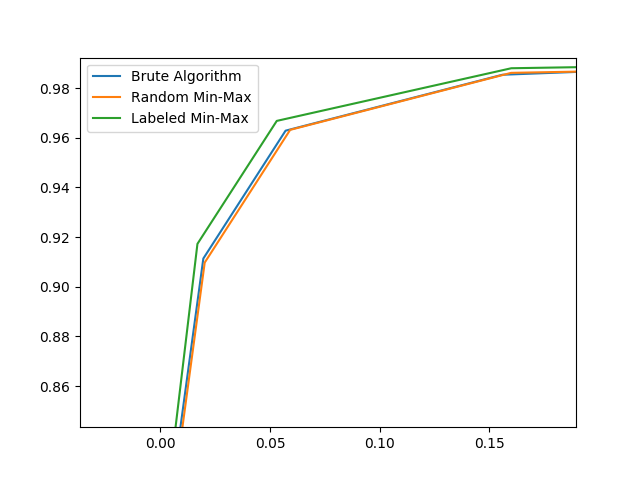
\includegraphics[width=.9\linewidth]{figure_1.png}



The time cost between serialized min-max and parallelized min-max is:

\begin{center}
\begin{tabular}{rlllll}
\hline
No. & Parallelized? & Algorithm & Trainning time & Testing time & Total time\\
\hline
1 & Yes & labeled & 59.37346 s & 144.54046 s & 203.93383 s\\
2 & No & labeled & 115.96271 s & 371.83840 s & 489.00508 s\\
3 & Yes & random & 54.49303 s & 84.16756 s & 138.69087 s\\
4 & No & random & 103.98813 s & 200.19163 s & 305.47026 s\\
\hline
\end{tabular}
\end{center}


Test environment is Ubuntu, 4 kernal.
Python version is 3.5.
% Emacs 24.5.1 (Org mode 8.2.10)
\end{document}